\documentclass{beamer}

\mode<presentation>
\usetheme{Antibes}

\usepackage[spanish]{babel}
\usepackage[utf8]{inputenc}
\usepackage[T1]{fontenc} % hyphenation 
\usepackage{times}
\usepackage{tikz}

\setbeamercovered{dynamic}

\title[QGIS]{Introducción a QGIS}
\subtitle[]{Curso de Zonificación Vitícola y Viticultura de Precisión}


\author[G.F. Olmedo]{Ing. Agr. Guillermo Federico Olmedo}

\institute[INTA] % (optional, but mostly needed)
{ Laboratorio de Geomática\\
  Recursos Naturales\\
  INTA EEA Mendoza\\
  \vskip10pt
\begin{columns}
	\column{.5\textwidth}
	\begin{flushright}
		
\includegraphics[width=1.7cm]{logoINTA}
	\end{flushright}
	\column{.5\textwidth}
	\begin{flushleft}
		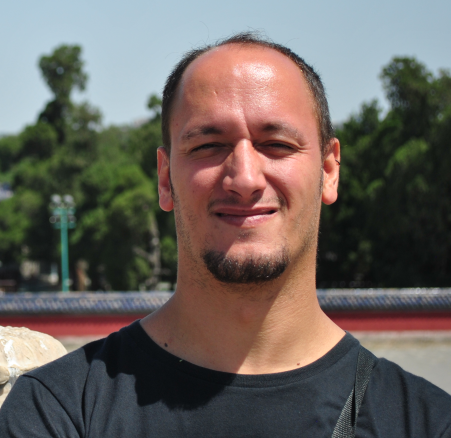
\includegraphics[width=1.7cm]{yo}
	\end{flushleft}
\end{columns}  
}

\date[FCA, 16-20/05/2016]{Fac. de Cs. Agrarias, 16 al 20 de mayo de 2016}

\pgfdeclareimage[height=0.5cm]{university-logo}{logoINTA}
\logo{\pgfuseimage{university-logo}}

%\beamerdefaultoverlayspecification{<+->}


\begin{document}

\begin{frame}[plain]
  \titlepage
\end{frame}

\begin{frame}{Outline}
	\tableofcontents[pausesections]
	% You might wish to add the option [pausesections]
\end{frame}

\section{Introducción}

\begin{frame}{¿Qué es QGIS?}
	\begin{itemize}[<+->]
		\item Es un completo Sistema de Información Geográfica y cliente de Infraestructura de Datos Espaciales.
		\item Capaz de acceder a los formatos más usuales tanto ráster como vectoriales. Integra datos tanto locales como remotos a través de estándares OGC, bases de datos geográficas, etc.
		\item Funcionalidades: Navegación, Consulta, Selección, Búsqueda, Geoprocesos, Edición gráfica y alfanumérica, Representación vectorial y raster, Etiquetado, Tablas, Constructor de mapas, Impresión, Redes, Raster y teledetección, Publicación, 3D y animación, Topología, gestión de Sistemas de Referencia Coordenados, exportar/importar WMC, scripting, gestión de traducciones, etc.
	\end{itemize}
\end{frame}

\begin{frame}{¿Qué se puede hacer con QGIS?}
	\begin{itemize}[<+->]
		\item Ver, editar y crear una gran variedad de formatos vectoriales como shapefiles, grass vectores, postgis, spaciallite \ldots
		\item Ver raster como TIFF, Erdas Img, Grass, \ldots
		\item Crear complementos a medida con Python
	\end{itemize}
\end{frame}

\begin{frame}{QGIS es extensible}
	\centering
	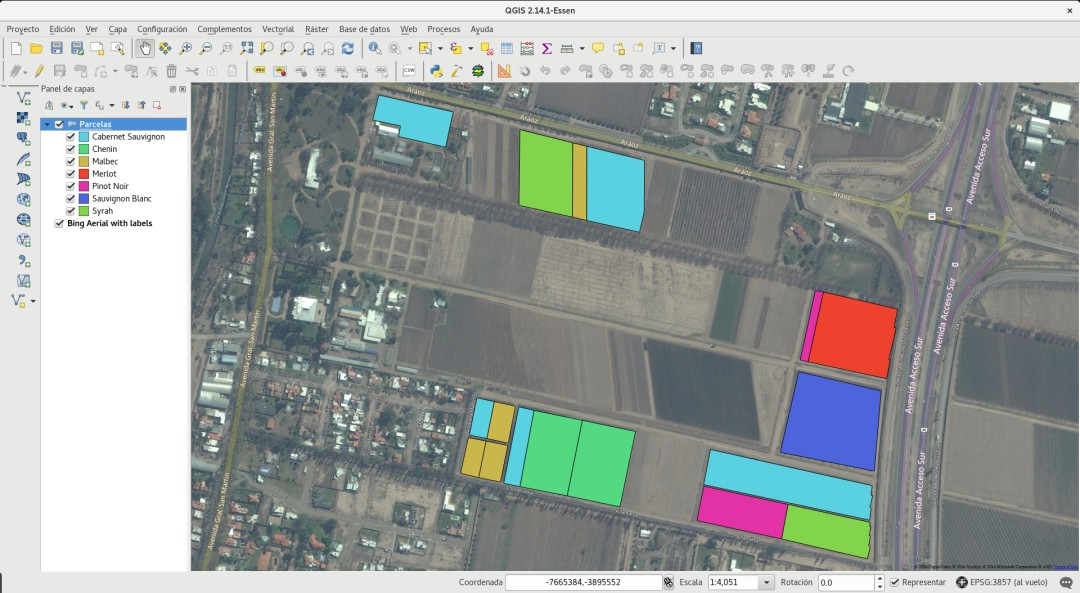
\includegraphics[width=1\textwidth]{QGIS+bing}
\end{frame}

\begin{frame}{QGIS es extensible}
	\centering
	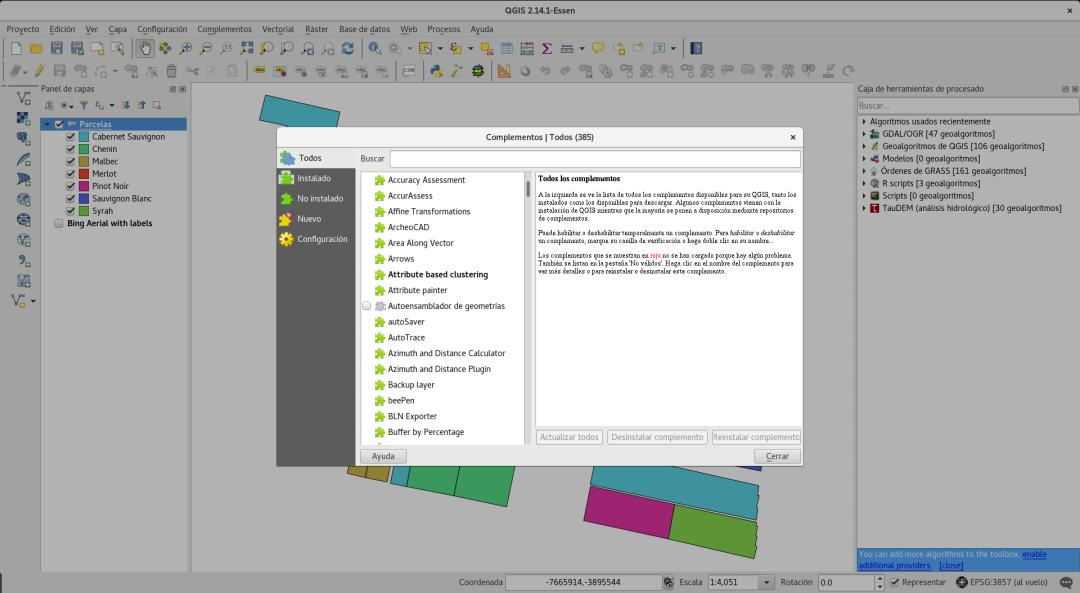
\includegraphics[width=1\textwidth]{QGIS-plugins}
\end{frame}



\section{Recorrido por las herramientas}

\begin{frame}{La interfaz de QGIS}
	\centering
	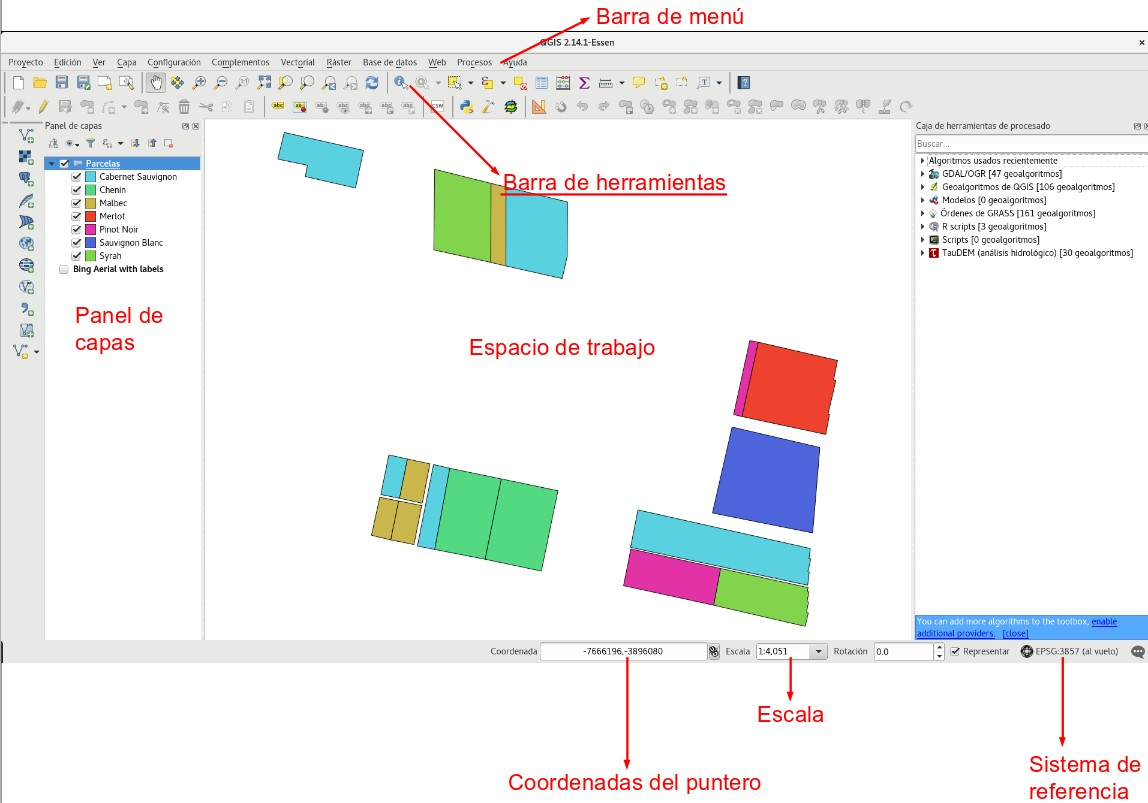
\includegraphics[width=0.8\textwidth]{interfaz}
\end{frame}

\begin{frame}{barras de herramientas}
	\centering
	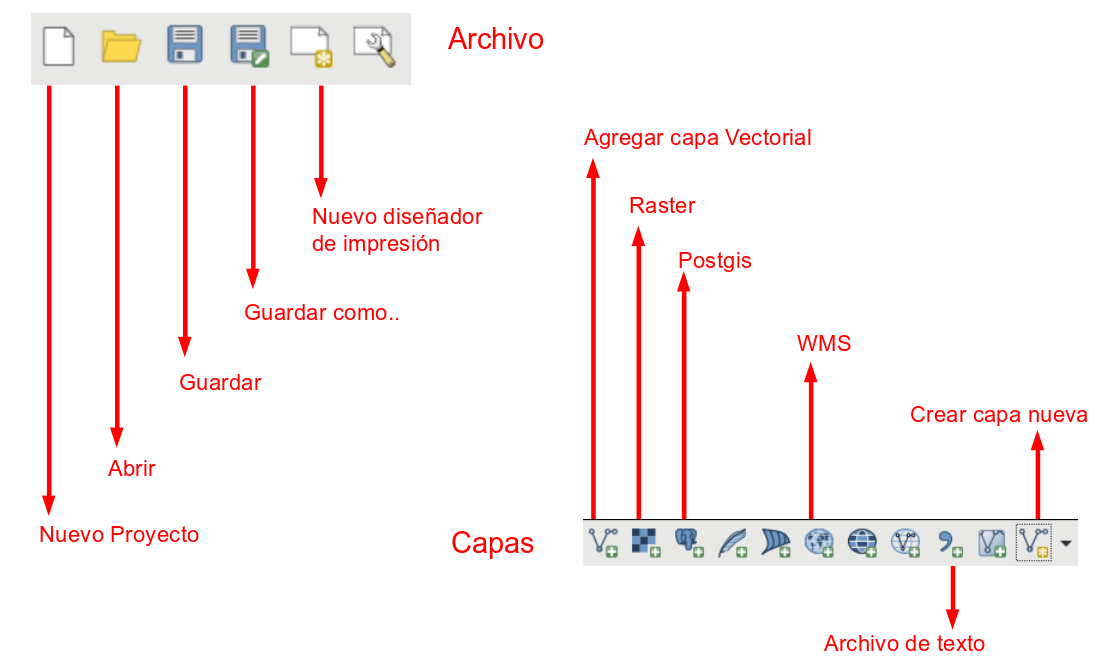
\includegraphics[width=1\textwidth]{tb1}
\end{frame}

\begin{frame}{barras de herramientas}
	\centering
	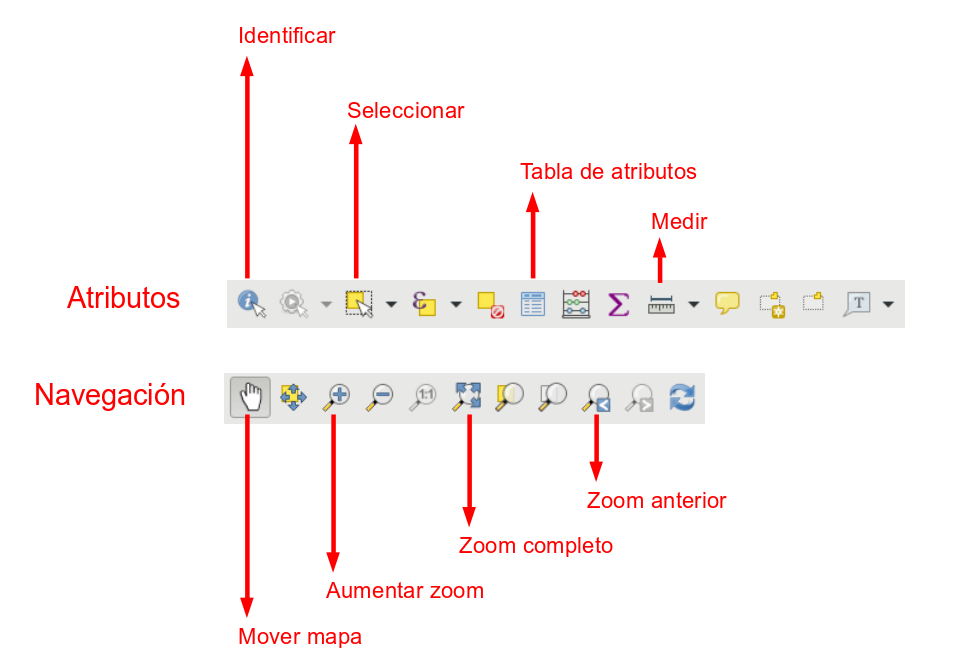
\includegraphics[width=0.9\textwidth]{tb2}
\end{frame}

\begin{frame}{barras de herramientas}
	\centering
	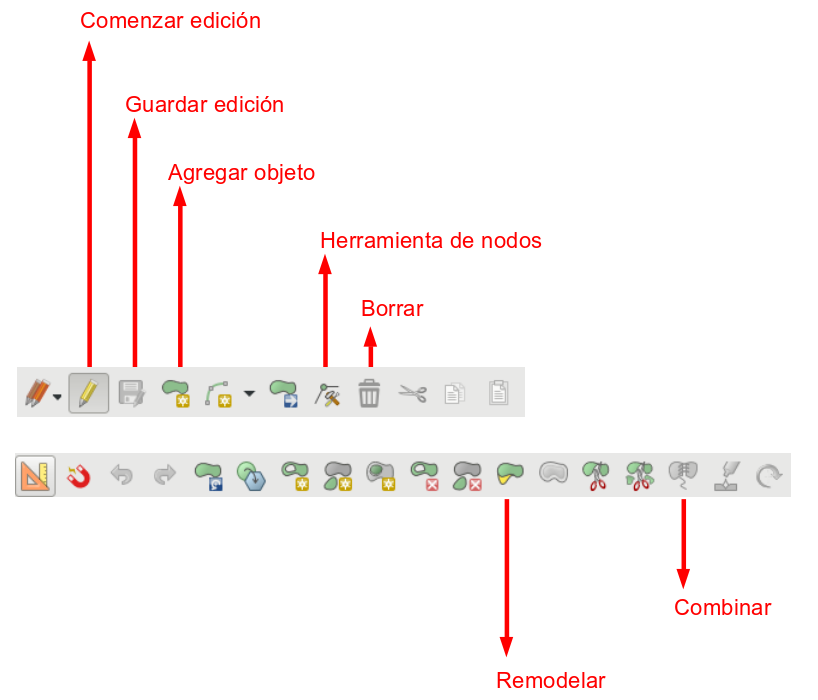
\includegraphics[width=0.8\textwidth]{tb3}
\end{frame}

\begin{frame}{La herramienta remodelar}
		    \begin{figure}
			    	\includegraphics<1>[width=0.8\textwidth]{rem1}
			    	\includegraphics<2>[width=0.8\textwidth]{rem2}
			    	\includegraphics<3>[width=0.8\textwidth]{rem3}
			    	\includegraphics<4>[width=0.8\textwidth]{rem4}
			    	\includegraphics<5>[width=0.8\textwidth]{rem5}
			    \end{figure} 
\end{frame}

\end{document}

